% -*- root: main.tex -*-

\chapter{Mapowanie obiektowe}

Jedną z~największych zalet relacyjnych baz danych w~kontekście programowania obiektowego jest dostępność bibliotek, które umożliwiają proste mapowanie obiektowo-relacyjne\footnote{W~dalszej części pracy używany będzie skrót ORM od angielskiego pojęcia object-relational mapping.}. Wykorzystanie ORM znacząco upraszcza proces tworzenia oprogramowania wykorzystującego bazy danych:

\begin{itemize}
	\item Umożliwia definiowanie modelu danych poprzez tworzenie klas reprezentujących obiekty wykorzystywane w~aplikacji.
	\item Zarządzanie połączeniami, sesjami i~transakcjami bazodanowymi jest znacząco uproszczone lub dokonywane automatycznie.
	\item Zwiększa bezpieczeństwo aplikacji. Mechanizmy ORM dostarczają narzędzi do ochrony przez atakami typu SQL Injection\footnote{SQL Injection (ang. wstrzykiwanie SQL) - typ ataku polegający na wykorzystywaniu specjalnie spreparowanych wartości, które dołączone do szablonu zapytania SQL powodują szkodliwe działania niezgodne z~intencją programisty.}.~\cite{orm_sql_injection_protection}
	\item Umożliwia modyfikacje środowiska bazodanowego bez zmieniania kodu aplikacji. Mechanizmy ORM wspierają wiele silników bazodanowych, które mogą różnić się od siebie implementowanymi standardami języka SQL. 
\end{itemize}

O~popularności mechanizmów ORM świadczy fakt powstawania oficjalnych standardów mapowania obiektowo-relacyjnego włączanych do specyfikacji języków programowania. Przykładem takiego standardu jest JPA\footnote{Java Persistence API.} dla języka Java.

\section{Mapowanie obiektowo-relacyjne dla Cassandry}

Wraz z~pojawieniem się języka CQL pojawiła się szansa wykorzystania istniejących implementacji mechanizmów ORM do przechowywania danych z~użyciem silnika Cassandry. Motywacją do stworzenia takiego rozwiązania jest zwiększenie wydajności istniejących aplikacji bez modyfikacji ich kodu. Minimalna rekonfiguracja aplikacji i~podłączenie jej pod klaster bazodanowy skutkowałyby zwiększeniem wydajności działania aplikacji. Ponadto wykorzystanie istniejących interfejsów mogłoby umożliwić obsługę różnych typów baz danych należących do ruchu NoSQL. 

Przykładem projektu, który wykorzystuje mechanizm ORM do obsługi NoSQLowych baz danych jest Kundera.\cite{kundera_home} Kundera zapewnia implementację mapowania obiektowego zgodną ze standardem JPA 2.0 między innymi dla Cassandry, HBase, MongoDB oraz Neo4j. Dodatkowo biblioteka wspiera obsługę wielu mechanizmów równocześnie.

\subsection{Wydajność}

Wyniki pomiarów na stronie domowej projektu Kundera świadczą o~tym, że biblioteka nie wprowadza znacznych narzutów wydajnościowych względem bezpośredniego wykorzystania interfejsu bazy danych. Ważniejsze jest jednak sprawdzenie jak duży narzut wprowadza dostosowanie relacyjnego modelu danych do Apache Cassandry. W~tym celu Autor przeprowadził testy porównawcze masowego wstawiania i~pobierania obiektów. Dla każdej z~dwóch operacji zostały przeprowadzone trzy testy. Pierwszy test mierzy czas referencyjny. Jest wykonywany dla zdenormalizowanego modelu Cassandry przedstawionego na diagramie~\ref{tab:denormalized_wishlist}. Drugi test sprawdza czasy dla znormalizowanego modelu zaprezentowanego na diagramie~\ref{fig:er_wishlist}, opisanego w~JPA i~uruchomiony na Cassandrze z~wykorzystaniem biblioteki Kundera. Trzeci test wykorzystuje identyczny opis modelu jak drugi, jednakże wykonywany jest dla silnika MySQL. Wszystkie testy przeprowadzane były jednowątkowo. Czas opóźnień przesyłania danych jest pomijalny, gdyż testy były prowadzone na środowisku lokalnym.

W~trakcie testów mierzony był całkowity czas wykonania danej operacji. Przyjęte zostały następujące założenia:

\begin{itemize}
	\item Liczba użytkowników i~przedmiotów są parametryzowane i~skalowane liniowo.
	\item Liczba przedmiotów, które użytkownik może mieć na swojej liście życzeń zawiera się w~przedziale $[0;10]$.
	\item Odczytywana jest parametryzowalna liczba użytkowników.
\end{itemize}

\noindent Wyniki czasu wstawiania wielu rekordów zostały przedstawione na wykresie~\ref{fig:insert_time_comparison}. Czasy pobierania wielu rekordów zostały zebrane na wykresie~\ref{fig:select_time_comparison}.

\begin{figure}
	\centering
	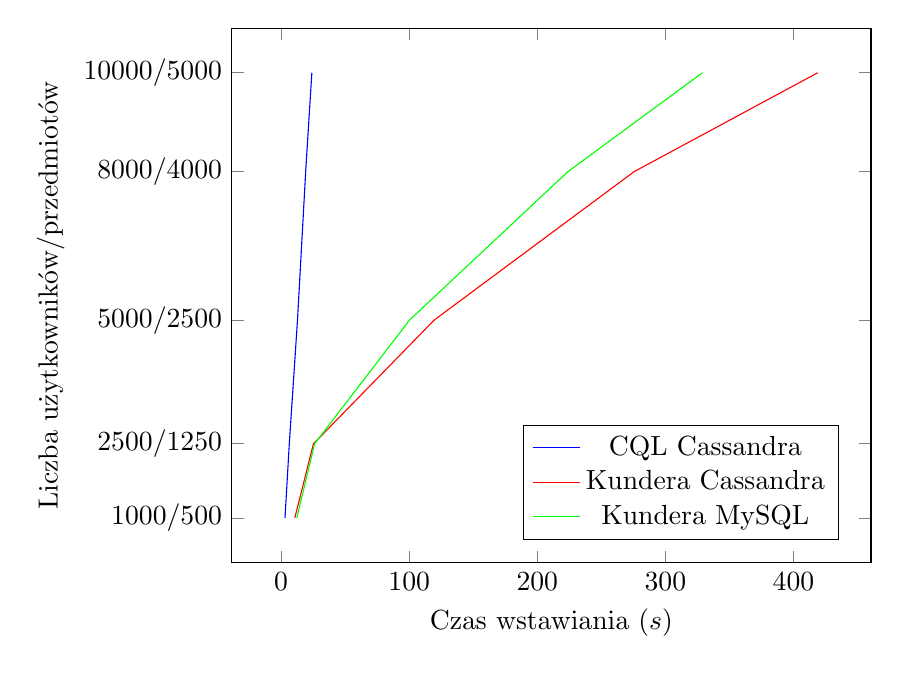
\begin{tikzpicture}
		\begin{axis}[
				width=.8\textwidth,
				xlabel=Czas wstawiania ($s$),
				ylabel=Liczba użytkowników/przedmiotów,
				scaled ticks=false, 
				tick label style={/pgf/number format/fixed},
				ytick={1000, 2500, 5000, 8000, 10000},
				yticklabels={1000/500, 2500/1250, 5000/2500, 8000/4000, 10000/5000},
				legend style={at={(0.95,0.15)},anchor=east}
			]
			\addplot[color=blue] coordinates {
				(23.978, 10000)
				(19.155, 8000)
				(12.762, 5000)
				(6.366, 2500)
				(3.005, 1000)
			};
			\addlegendentry{CQL Cassandra}

			\addplot[color=red] coordinates {
				(418.915, 10000)
				(275.532, 8000)
				(119.453, 5000)
				(25.213, 2500)
				(10.657, 1000)
			};
			\addlegendentry{Kundera Cassandra}

			\addplot[color=green] coordinates {
				(328.915, 10000)
				(223.823, 8000)
				(100.23, 5000)
				(26.119, 2500)
				(12.232, 1000)
			};
			\addlegendentry{Kundera MySQL}
		\end{axis}
	\end{tikzpicture}

	\caption{Porównanie czasu wstawiania wielu rekordów.}
	\label{fig:insert_time_comparison}
\end{figure}

\begin{figure}
	\centering
	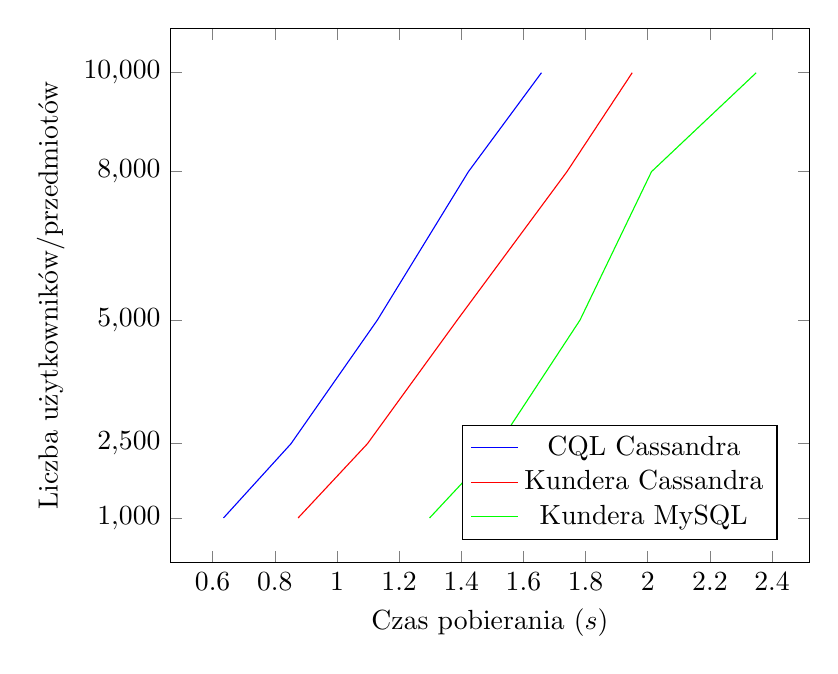
\begin{tikzpicture}
		\begin{axis}[
				width=.8\textwidth,
				xlabel=Czas pobierania ($s$),
				ylabel=Liczba użytkowników/przedmiotów,
				scaled ticks=false, 
				tick label style={/pgf/number format/fixed},
				ytick={1000, 2500, 5000, 8000, 10000},
				legend style={at={(0.95,0.15)},anchor=east}
			]
			\addplot[color=blue] coordinates {
				(1.658, 10000)
				(1.423, 8000)
				(1.130, 5000)
				(0.852, 2500)
				(0.635, 1000)
			};
			\addlegendentry{CQL Cassandra}

			\addplot[color=red] coordinates {
				(1.95, 10000)
				(1.74, 8000)
				(1.387, 5000)
				(1.098, 2500)
				(0.875, 1000)
			};
			\addlegendentry{Kundera Cassandra}

			\addplot[color=green] coordinates {
				(2.349, 10000)
				(2.012, 8000)
				(1.782, 5000)
				(1.521, 2500)
				(1.298, 1000)
			};
			\addlegendentry{Kundera MySQL}
		\end{axis}
	\end{tikzpicture}

	\caption{Porównanie czasu pobierania wielu rekordów.}
	\label{fig:select_time_comparison}
\end{figure}

Wyniki zebrane na wykresie~\ref{fig:insert_time_comparison} pokazują, że wykorzystanie mechanizmów mapowania obiektowo-relacyjnego dla bazy danych Cassandra jest bardzo złym wyborem. Narzut związany z~konwersją modelu danych do postaci relacyjnej jest tak duży, że w~praktyce pojedynczy węzeł Cassandry osiąga gorsze wyniki zapisu niż baza danych MySQL. Zmiana silnika bazodanowego dla istniejącego kodu nie tylko nie poprawi wyników wydajnościowych, ale może wręcz spowodować spowolnienie działania aplikacji. Jedynym zyskiem z~takiego rozwiązania będzie możliwość wykorzystania natywnego mechanizmu klastrowania węzłów Cassandry. Dzięki temu wyeliminowany zostanie pojedynczy punkt awarii systemu. Ten sam efekt można jednak uzyskać stosując rozwiązana dedykowane dla relacyjnych baz danych. Przykładami takich rozwiązań mogą być MySQL Cluster CGE dla bazy danych MySQL oraz Oracle RAC dla baz Oracle Database Enterprise Edition.

Potencjalnym zastosowaniem mapowania obiektowo-relacyjnego dla bazy danych Cassandra są środowiska integracyjne dla wielu aplikacji. Wykorzystując homogeniczny model danych można odwoływać się do różnych silników bazodanowych. W~bibliotece Kundera istnieje takie rozwiązane. Zostało nazwane Polyglot Persistence\footnote{Polyglot Persistence (dosłowne tłumaczenie to ,,zapis poliglotyczny'') - opis mechanizmu znajduje się na stronie \url{https://github.com/impetus-opensource/Kundera/wiki/Polyglot-Persistence}.}. W~praktyce dostosowanie modelu danych ORM do istniejących schematów baz danych jest problematyczne.  

Wykres~\ref{fig:insert_time_comparison} demonstruje jak ogromną przewagę szybkości przy zapisie posiada poprawnie zaprojektowany model danych Apache Cassandra. Przypuszczalnie osiągnięty czas mógłby być jeszcze lepszy, gdyż ograniczenie wydajności zapisu nastąpowało prawdopodobnie po stronie klienta testowego. Zgodnie ze specyfikacją Apache Cassandra jest w~stanie obsługiwać bez opóźnień znacznie więcej jednoczesnych żądań zapisu.

Czasy pobierania listy życzeń użytkownika przedstawione na wykresie~\ref{fig:select_time_comparison} nie różnią się znacząco od siebie. Przewaga szybkości pobierania danych z~wykorzystaniem CQL ponownie wynika z~zastosowania lepszego modelu danych. Denormalizacja pól encji \emph{Item} pozwala pominąć pobieranie dla każdego użytkownika dodatkowego wiersza z~bazy danych. 